\section{Basic definitions}
\begin{frame}
  \frametitle{What is Skeletonization?}
  \begin{block}{Skeletonization}
    An image processing technique which reduces a binary object (or region) to a 1 pixel wide representation called \textbf{skeleton}.
  \end{block}
  Useful in many application fields such as \emph{shape recognition and analysis}, \emph{animation}, \emph{motion tracking} or \emph{medical imaging}~\cite{skel-applications}.
  \begin{figure}
    \begin{center}
      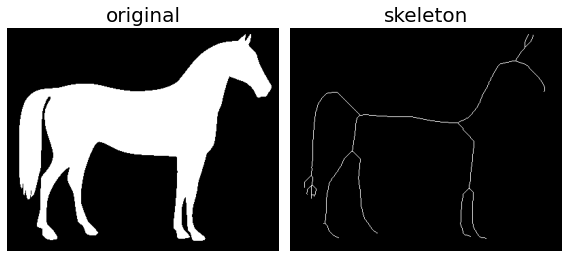
\includegraphics[width=0.6\textwidth]{skeletonization-example.png}
      \caption{Example of a skeletonized image.}
    \end{center}
  \end{figure}
\end{frame}

\begin{frame}
  \label{sli:skeleton}
  \frametitle{What is Skeletonization?}
  \begin{block}{Skeleton}
    The ideal skeleton should:
    \begin{itemize}
      \item be a \textbf{connected subset} of points from the original region,
      \item represent the \textbf{geometric} characteristics of the region (e.g. area, curvature...),
      \item preserve the \textbf{topological} characteristics of the region (e.g. connectivity, holes, cavities...)
    \end{itemize}
  \end{block}

  Three major skeletonization techniques:
  \begin{itemize}
    \item Medial-axis distance transform
    \item Non-pixel-based methods (computes analytically the skeleton)
    \item Thinning methods
  \end{itemize}
  \vspace{0.5cm}
  We will focus on \textbf{thinning methods} since they are quite efficient and commonly used in state-of-the-art applications.
\end{frame}
